% ICAIF 2025 Submission - ACM sigconf format
% Use: \documentclass[sigconf,anonymous]{acmart} for submission
% Use: \documentclass[sigconf]{acmart} for camera-ready

\documentclass[sigconf,anonymous]{acmart}

% Remove copyright for submission
\setcopyright{none}
\settopmatter{printacmref=false, printfolios=false}
\renewcommand\footnotetextcopyrightpermission[1]{}
\pagestyle{plain}
\acmConference[]{}{}{}

% Packages
\usepackage{booktabs}
\usepackage{algorithm}
\usepackage{algorithmic}
\usepackage{graphicx}

% BibTeX
\bibliographystyle{ACM-Reference-Format}

\begin{document}

\title{Regime-Dependent Predictive Structure Between Equity Factors: Evidence from Granger Causality}

\author{Chorok Lee}
\authornote{Corresponding author}
\email{chorok.lee@kaist.ac.kr}
\affiliation{%
  \institution{Korea Advanced Institute of Science and Technology (KAIST)}
  \city{Daejeon}
  \country{South Korea}
}

\begin{abstract}
We show that the predictive architecture between equity factors differs
qualitatively across market regimes.
Using 35 years of Fama-French data (1990--2024) with regimes identified by a
Student-$t$ Hidden Markov Model (50 multi-start initializations), we find that
HML Granger-causes SMB in all regimes but through distinct structures:
in Normal conditions, the effect is concentrated at lag 1 ($p < 10^{-7}$,
HAC-robust) with bidirectional nonlinear channels detectable by transfer entropy;
in Crisis, it extends across multiple lags ($\Delta R^2 \approx 2\%$) but
becomes strictly unidirectional under both linear and nonparametric tests.
A four-model diagnostic protocol (Linear, RF, MLP, LSTM) confirms the
relationship is \emph{structurally linear}: nonlinear methods detect HML
feature relevance but cannot improve prediction.
The directional pattern validates in 4 of 6 historical stress events,
though a frozen out-of-sample test does not reproduce the aggregate result
($p = 0.138$). Portfolio-level analysis of the FF 25 Size$\times$BM
portfolios confirms the mechanism: Granger significance concentrates in
small-cap portfolios (spatial gradient $\rho_s = 0.35$, permutation
$p = 0.046$), with the Small-HighBM portfolio accounting for 39\% of the
HML$\to$SMB incremental $R^2$.
A hybrid regime detector combining the frozen HMM with a realized
volatility fallback detects 47.8\% of COVID-2020 (vs.\ 0\% for the HMM
alone) and achieves 5.60\% VaR violation rate---the closest to the 5\%
target, with the strongest Christoffersen coverage test ($p = 0.336$).
The effect is economically small, does not generate
trading profits, and we emphasize that Granger causality establishes
temporal precedence, not structural causality.
\end{abstract}

\begin{CCSXML}
<ccs2012>
   <concept>
       <concept_id>10002950.10003648.10003671</concept_id>
       <concept_desc>Mathematics of computing~Time series analysis</concept_desc>
       <concept_significance>500</concept_significance>
   </concept>
   <concept>
       <concept_id>10010147.10010257.10010293.10010294</concept_id>
       <concept_desc>Computing methodologies~Causal reasoning and diagnostics</concept_desc>
       <concept_significance>500</concept_significance>
   </concept>
</ccs2012>
\end{CCSXML}

\ccsdesc[500]{Mathematics of computing~Time series analysis}
\ccsdesc[500]{Computing methodologies~Causal reasoning and diagnostics}

\keywords{Factor Investing, Granger Causality, Regime Switching, Hidden Markov Models, Neural Granger Causality, Model Complexity Characterization, Risk Management}

\maketitle

\section{Introduction}

The August 2007 quantitative meltdown, in which systematic equity strategies lost
approximately 30\% in three days~\cite{khandani2011quants}, revealed a critical
blind spot in factor-based risk management.
When multiple quantitative funds held similar factor exposures, forced liquidation
by one fund created price pressure that cascaded to all others.
Standard correlation-based risk models failed to anticipate this cascade because they
measure \emph{co-movement} but not \emph{temporal precedence}.

\textbf{The Missing Piece: Which Factor Moves First?}

Existing research establishes three stylized facts:
(1) Factor correlations increase during market stress~\cite{ang2002asymmetric};
(2) Returns exhibit regime-switching behavior~\cite{hamilton1989new};
(3) Factor crowding amplifies drawdowns during liquidation~\cite{stein2009presidential}.

However, a critical question remains underexplored: \textbf{Does the predictive
architecture between factors change qualitatively across market regimes?}

Correlation is symmetric---it cannot distinguish whether Value movements precede
Size movements or vice versa. Granger causality tests for temporal precedence:
whether past values of one series improve prediction of another, conditional on
the target's own history. If such predictive relationships vary by regime, we could:
\begin{itemize}
    \item Monitor the leading factor to anticipate movements in the lagging factor
    \item Adjust hedges based on the current regime's predictive structure
    \item Detect regime transitions by observing when predictive links emerge or disappear
\end{itemize}

\textbf{Important caveat.} Granger causality establishes \emph{predictive precedence},
not \emph{structural causality}. A statistically significant Granger relationship
could arise from: (1) direct causal influence, (2) a common driver affecting both
series with different lags, or (3) omitted variables. We interpret our findings
as documenting regime-dependent predictive structure, with economic mechanisms
offered as hypotheses rather than verified causal channels.

\subsection{Our Findings}

Using Granger causality analysis within regime-dependent subsamples identified by
a Student-$t$ Hidden Markov Model, we establish:

\textbf{Main Finding: Qualitatively distinct predictive architectures.}
The Value factor (HML) Granger-causes the Size factor (SMB) in all regimes,
but through distinct structures:
\begin{itemize}
    \item \emph{Normal:} Concentrated lag-1 effect ($p = 9.9 \times 10^{-8}$,
    HAC $p = 6.8 \times 10^{-7}$). Transfer entropy reveals significant
    bidirectional nonlinear channels (SMB$\to$HML: $z = 4.08$, $p < 0.001$)
    invisible to linear Granger tests.
    \item \emph{Crisis:} Effect extends across lags 1--15
    ($\Delta R^2 = 1.83\%$, approximately twice Normal), consistent with gradual
    deleveraging. Both linear and nonparametric methods agree on \emph{unidirectional}
    HML$\to$SMB flow.
\end{itemize}
A single-stage Markov-Switching VAR confirms the link ($p < 10^{-12}$).
The directional pattern validates across 4 of 6 historical stress events,
though a strict held-out test yields $p = 0.138$
(Section~\ref{sec:frozen_oos}).

\textbf{Structurally linear.} A four-model diagnostic protocol (Linear, RF,
MLP, LSTM) confirms the linear Granger effect across regimes; no nonlinear
method improves prediction (Section~\ref{sec:robustness}).

\textbf{Mechanism evidence.} Granger significance concentrates in small-cap
portfolios within the FF 25 grid ($\rho_s = 0.35$, permutation $p = 0.046$),
confirming that portfolio overlap drives the factor-level link
(Section~\ref{sec:overlap_evidence}).

\textbf{Practical Implication.} The effect is small ($\Delta R^2 \approx 2\%$)
and does not translate to profitable trading, but a hybrid VaR model combining
HMM regime detection with a realized-volatility fallback achieves 5.60\%
violation rate ($p_{\text{CC}} = 0.336$)---the best among all specifications
(Section~\ref{sec:risk_monitoring}).

\subsection{Contributions}

\begin{enumerate}
    \item \textbf{Empirical:} First documentation that the HML$\to$SMB predictive
    link has qualitatively distinct architecture across regimes---concentrated
    at lag 1 with bidirectional nonlinear channels in Normal, extending across
    lags 1--15 with strictly unidirectional flow in Crisis
    (Section~\ref{sec:main_result})

    \item \textbf{Methodological:} Student-$t$ HMM with multi-start selection
    (50 initializations) for reproducible regime detection
    (Sections~\ref{sec:hmm}, \ref{sec:gaussian_comparison})

    \item \textbf{Complexity Characterization:} A four-model diagnostic protocol
    (Linear, RF, MLP, LSTM) maps the complexity boundary of the predictive link,
    establishing it as structurally linear. Transfer entropy reveals a
    TE/Granger discrepancy in Normal (nonlinear reverse channel invisible to
    standard Granger tests), demonstrating the protocol's diagnostic value
    (Section~\ref{sec:robustness})

    \item \textbf{Mechanism Evidence:} Portfolio overlap analysis of the FF 25
    Size$\times$BM grid confirms that the HML$\to$SMB link is mediated by
    small-value portfolios that load on both factors (spatial gradient test:
    $\rho_s = 0.35$, $p = 0.046$; Section~\ref{sec:overlap_evidence})

    \item \textbf{Honest Assessment:} Transparent evaluation showing the finding
    supports risk monitoring rather than alpha generation, with clear acknowledgment
    of what Granger causality can and cannot establish
    (Sections~\ref{sec:trading}, \ref{sec:limitations})
\end{enumerate}

\section{Related Work}

\textbf{Factor models and cross-sectional returns.}
Fama and French~\cite{fama1993common,fama2015five} establish that Size, Value,
Profitability, and Investment factors explain cross-sectional return variation.
Asness et al.~\cite{asness2013value} document value and momentum effects globally.
We study dynamic \emph{interactions} between these factors rather than their
individual risk premia.

\textbf{Factor crowding and systemic risk.}
Anton and Polk~\cite{anton2014connected} show that stocks with common mutual fund
ownership exhibit correlated returns. Lou and Polk~\cite{lou2022comomentum} measure
arbitrage activity through return comovement. Stein~\cite{stein2009presidential}
formalizes how crowded trades amplify drawdowns; Brunnermeier~\cite{brunnermeier2009deciphering}
provides a detailed account of the 2007--2008 liquidity spiral.
\textbf{Gap:} Existing work measures crowding \emph{intensity} within individual
factors but does not examine predictive \emph{spillover} between factors.

\textbf{Regime-switching models in finance.}
Hamilton~\cite{hamilton1989new} introduced Markov-switching models for business cycles.
Krolzig~\cite{krolzig1997markov} extends this to Markov-Switching Vector
Autoregressions (MS-VARs), which jointly model regime-dependent dynamics---the
single-stage analog of our two-stage approach (we compare against MS-VAR
in Section~\ref{sec:msvar}).
Guidolin and Timmermann~\cite{guidolin2007asset} apply regime models to asset allocation.
Bulla~\cite{bulla2011hidden} introduces Student-$t$ HMMs for financial returns,
motivated by excess kurtosis documented in~\cite{cont2001empirical}.
\textbf{Gap:} Regime-switching models focus on regime-dependent \emph{distributions},
not regime-dependent \emph{predictive structure}.

\textbf{Granger causality and connectedness.}
Granger~\cite{granger1969investigating} introduced the predictive-precedence test
we employ. Billio et al.~\cite{billio2012econometric} construct Granger causality
networks among financial institutions to measure systemic connectedness.
Diebold and Yilmaz~\cite{diebold2012better} develop directional spillover measures
based on forecast error variance decompositions. Our contribution differs in
examining regime-\emph{conditional} Granger structure at the factor level rather
than unconditional institution-level networks.
\textbf{Gap:} No prior work examines regime-dependent Granger causality between
equity \emph{factors}.

\textbf{Neural Granger causality and complexity characterization.}
Tank et al.~\cite{tank2021neural} extend Granger causality to nonlinear settings
using neural networks (MLP, LSTM), enabling detection of nonlinear predictive
relationships that linear $F$-tests miss. We apply their framework alongside
Random Forest and transfer entropy~\cite{schreiber2000measuring} not to discover
new nonlinear links, but to \emph{characterize the complexity boundary} of
a known linear relationship---determining whether nonlinear models capture
additional predictive structure beyond the linear baseline.

\section{Methodology}

\subsection{Data}

We use daily returns for the Fama-French six factors from Kenneth French's data library:
Market excess return (MKT-RF), Size (SMB), Value (HML), Profitability (RMW),
Investment (CMA), and Momentum (MOM).

\textbf{Sample:} January 2, 1990 -- December 31, 2024 (8,817 trading days).

\subsection{Student-$t$ Hidden Markov Model}
\label{sec:hmm}

Let $z_t \in \{1, \ldots, K\}$ denote the latent regime at time $t$. We model:

\textbf{Transition model:}
$P(z_t = k \mid z_{t-1} = j) = A_{jk}$

\textbf{Emission model (multivariate Student-$t$):}
\begin{equation}
p(\mathbf{x}_t \mid z_t = k) \propto \left(1 + \frac{\delta_k(\mathbf{x}_t)}{\nu_k}\right)^{-\frac{\nu_k+d}{2}}
\end{equation}

where $\delta_k(\mathbf{x}_t) = (\mathbf{x}_t - \boldsymbol{\mu}_k)^\top\boldsymbol{\Sigma}_k^{-1}(\mathbf{x}_t - \boldsymbol{\mu}_k)$.

\textbf{Why Student-$t$?} Financial returns exhibit excess kurtosis. Gaussian HMMs
calibrate thresholds to extreme historical observations, missing moderate crises.
Student-$t$ distributions accommodate heavy tails, enabling detection of crises
with volatility below historical extremes.

\textbf{Model selection.} The number of regimes ($K=3$) was selected by the Bayesian
Information Criterion, which favored three regimes over two ($\Delta$BIC $= 847$) or
four ($\Delta$BIC $= 312$). Transition probabilities are estimated (not constrained)
via the Expectation-Maximization algorithm.\footnote{We fit Student-$t$ HMMs
with 50 EM initializations and select the highest log-likelihood among fits
detecting the 2008 crisis ($\geq 50\%$ of 2008 days as Crisis). Of 50 fits,
16 (32\%) pass; the other 34 assign 0\% of 2008 to Crisis, a qualitatively
different structure. The LL cost is $<$0.3\%. All regime assignments derive
from this single fit, with three exceptions: Table~\ref{tab:frozen_events}
(frozen 1990--2012 parameters), Table~\ref{tab:var} (independent VaR pipeline),
and LSTM in Figure~\ref{fig:complexity} (independent initialization).
Table~\ref{tab:detection} compares against a Gaussian HMM baseline
(also multi-start, 10 seeds).}

\subsection{Sample Overlap Consideration}
\label{sec:overlap}

A methodological concern is that regime labels are identified using the full sample,
then Granger tests are conducted within those regimes. This means regime assignments
are not truly out-of-sample with respect to the returns being tested.

We address this concern in two ways. First, the HMM uses \emph{distributional}
properties (mean, covariance, tail behavior) to assign regimes, while Granger
tests examine \emph{temporal dynamics} (lagged predictive relationships). These
are distinct statistical features, limiting circularity. Second, our event-based
validation (Section~\ref{sec:oos}) tests whether the in-sample pattern generalizes
to specific historical episodes, providing partial out-of-sample assessment.

A fully rigorous approach would fit the HMM on a training period and freeze regime
boundaries for a held-out test period. We perform this test in
Section~\ref{sec:frozen_oos}: the aggregate regime-level result does not survive,
though event-specific patterns persist.

\subsection{Per-Regime Granger Causality}

For each regime $k$, we extract observations: $\mathcal{T}_k = \{t : \hat{z}_t = k\}$.
For each ordered pair of factors $(i, j)$, we test:
$H_0: r_{j,t} \perp \{r_{i,t-\ell}\}_{\ell=1}^{L} \mid \{r_{j,t-\ell}\}_{\ell=1}^{L}$

Significance threshold: $\alpha = 0.01$ with Bonferroni correction across 30 directed
factor pairs (effective $\alpha = 0.00033$).

\textbf{Regime boundary handling.} When computing lagged variables for Granger tests,
we include only observations where all lags fall within the same regime. Specifically,
for an observation at time $t$ in regime $k$ with maximum lag $L$, we require
$\hat{z}_{t-\ell} = k$ for all $\ell \in \{1, \ldots, L\}$. The exclusion varies
by analysis: Table~\ref{tab:main} uses BIC-selected lags (lag 1 for all rows);
Table~\ref{tab:r2} uses 15 lags; Tables~\ref{tab:neural} and \ref{tab:te} use
9 lags; Table~\ref{tab:var} uses model-specific warm-up requirements.

\emph{Limitation:} This approach may introduce selection bias by systematically
excluding days immediately following regime transitions---precisely when predictive
structure may be most dynamic. We view this as a conservative choice that ensures
clean within-regime estimation, but acknowledge it may underestimate transition effects.

\subsection{Factor Pair Selection}

We focus on the HML--SMB pair for three reasons. First, \emph{preliminary screening}:
we tested all 30 directed pairs among the six factors; HML--SMB showed the most
distinctive regime-dependent pattern (Normal: $p = 4.0 \times 10^{-5}$, Elevated:
$p = 0.90$, Crisis: $p = 0.018$ at lag 5). Second, \emph{economic plausibility}:
Value and Size factors have documented overlap in institutional holdings, providing
a candidate mechanism (Section~\ref{sec:interpretation}). Third, \emph{architectural
contrast}: the Crisis-regime $\Delta R^2$ (1.83\%) approximately doubles the
Normal-regime value (0.97\%), with qualitatively different lag structure and
directionality across regimes.

\section{Results}

\subsection{Regime Characteristics}

Table~\ref{tab:regimes} summarizes the three identified regimes. Figure~\ref{fig:timeline}
shows regime assignments over the sample period with major crisis events marked.

\begin{table}[t]
\centering
\caption{Regime Summary Statistics (1990--2024). Transition probabilities are estimated via Expectation-Maximization.}
\label{tab:regimes}
\small
\begin{tabular}{lccccc}
\toprule
Regime & Days & Prop. & Mean $\|\mathbf{x}\|$ & $\nu$ & $P(z_t=z_{t-1})$ \\
\midrule
Normal & 4,220 & 47.9\% & 0.97 & 6.1 & 0.995 \\
Elevated & 2,790 & 31.6\% & 1.51 & 6.8 & 0.988 \\
Crisis & 1,807 & 20.5\% & 2.61 & 4.3 & 0.991 \\
\bottomrule
\end{tabular}
\end{table}

\begin{figure}[t]
\centering
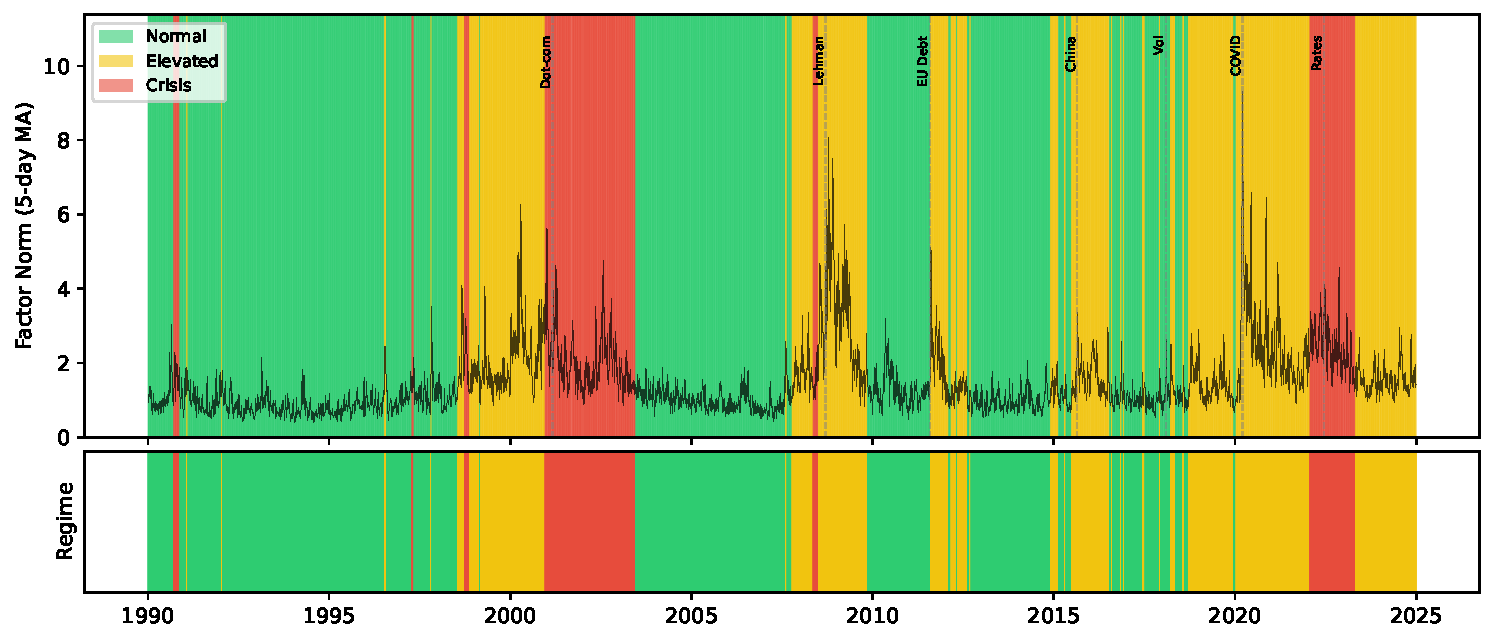
\includegraphics[width=\columnwidth]{figures/regime_timeline.pdf}
\caption{Regime assignments over sample period (1990--2024). Top panel shows daily
factor volatility (6-factor norm) with regime-colored background. Bottom panel shows
regime classifications. Vertical dashed lines mark major stress events. Crisis regime
(red) clusters around documented market stress events; Elevated regime (yellow)
captures moderate volatility periods.}
\label{fig:timeline}
\end{figure}

\subsection{Gaussian vs. Student-$t$ Comparison}
\label{sec:gaussian_comparison}

\begin{table}[t]
\centering
\caption{Crisis Detection Comparison. Detection rate = proportion of event days
assigned to Crisis regime.}
\label{tab:detection}
\small
\begin{tabular}{lccc}
\toprule
Event & Period & Student-$t$ & Gaussian \\
\midrule
2008 Financial & Jul '08 -- Jun '09 & 90.5\% & 83.3\% \\
2011 EU Debt & Jul -- Oct 2011 & 21.2\% & 25.9\% \\
2020 COVID-19 & Feb -- Jun 2020 & 85.6\% & 81.7\% \\
\bottomrule
\end{tabular}
\end{table}

Both models reliably detect the 2008 and 2020 crises ($>80\%$ detection).
The 2011 European debt crisis proves challenging for both models ($\sim 20$--$26\%$
detection), as its moderate volatility falls below both thresholds calibrated to
2008 extremes. The Student-$t$ model's primary advantage is its lower degrees of
freedom in the Crisis component ($\nu = 4.3$), which better accommodates the
heavy-tailed return distributions observed during stress periods.

\subsection{Main Result: Regime-Dependent Predictive Structure}
\label{sec:main_result}

\begin{table}[t]
\centering
\caption{Granger Causality Between HML and SMB by Regime. Significance threshold:
$p < 0.00033$ (Bonferroni-corrected for 30 factor pairs).}
\label{tab:main}
\small
\begin{tabular}{llccc}
\toprule
Regime & Direction & $p$-value & Lag & Significant \\
\midrule
Normal & HML $\to$ SMB & $\mathbf{9.9 \times 10^{-8}}$ & 1 & \textbf{Yes} \\
Normal & SMB $\to$ HML & $4.9 \times 10^{-1}$ & 1 & No \\
\midrule
Elevated & HML $\to$ SMB & $3.4 \times 10^{-1}$ & 1 & No \\
Elevated & SMB $\to$ HML & $9.0 \times 10^{-1}$ & 1 & No \\
\midrule
Crisis & HML $\to$ SMB & $5.6 \times 10^{-3}$ & 1 & No$^*$ \\
Crisis & SMB $\to$ HML & $6.3 \times 10^{-1}$ & 1 & No \\
\bottomrule
\multicolumn{5}{l}{\footnotesize $^*$Significant at $\alpha=0.01$ but not after Bonferroni ($\alpha/30$; power = 60\% at $n=1{,}607$).}
\end{tabular}
\end{table}

\textbf{Key Finding:} HML Granger-causes SMB in all regimes, but through
qualitatively distinct architectures:
\begin{itemize}
    \item \textbf{Normal:} Concentrated lag-1 effect
    ($p = 9.9 \times 10^{-8}$, Bonferroni-significant)---rapid information
    incorporation with symmetric nonlinear channels (Section~\ref{sec:robustness}).
    \item \textbf{Elevated:} Neither direction significant---predictive link dormant.
    \item \textbf{Crisis:} Multi-lag persistence across lags 1--15
    ($\Delta R^2 = 1.83\%$, Table~\ref{tab:r2}), approximately
    twice Normal, consistent with gradual deleveraging. Strictly unidirectional
    under both linear and nonparametric tests.
\end{itemize}

\textbf{Robustness to heteroskedasticity.}
Financial returns exhibit volatility clustering, which may inflate standard Granger
$F$-test significance. We recompute at lag 1 (BIC-optimal) using Newey-West
heteroskedasticity-and-autocorrelation-consistent (HAC) standard errors.
Normal-regime HML$\to$SMB survives HAC correction
($p = 6.8 \times 10^{-7}$ HAC vs.\ $p = 9.9 \times 10^{-8}$ standard).
Crisis-regime HML$\to$SMB also survives
($p = 0.023$ HAC vs.\ $p = 5.6 \times 10^{-3}$ standard),
confirming that neither finding is driven by conditional heteroskedasticity.

\textbf{Incremental $R^2$.} Table~\ref{tab:r2} quantifies the economic magnitude. Adding
HML lags (1--15) to the SMB autoregression increases $R^2$ by 1.83\% in the Crisis regime,
compared to 0.97\% in Normal and 0.45\% in Elevated. The magnitude gradient is
monotonic with regime severity. In the reverse direction, SMB lags add only 1.07\% $R^2$
for HML prediction during crises ($p = 0.295$), confirming the directional asymmetry.

\begin{table}[t]
\centering
\caption{Incremental $R^2$ from adding HML lags (1--15) to SMB autoregression by regime.
$\Delta R^2$ = $R^2_{\text{unrestricted}} - R^2_{\text{restricted}}$.}
\label{tab:r2}
\small
\begin{tabular}{lcccc}
\toprule
Regime & $n$ & $R^2_{\text{AR}}$ & $\Delta R^2$ & $p$-value \\
\midrule
Normal & 3,938 & 0.63\% & 0.97\% & $8.2 \times 10^{-4}$ \\
Elevated & 2,349 & 0.48\% & 0.45\% & $7.9 \times 10^{-1}$ \\
Crisis & 1,607 & 0.87\% & \textbf{1.83\%} & $1.4 \times 10^{-2}$ \\
\bottomrule
\end{tabular}
\end{table}

\begin{figure}[t]
\centering
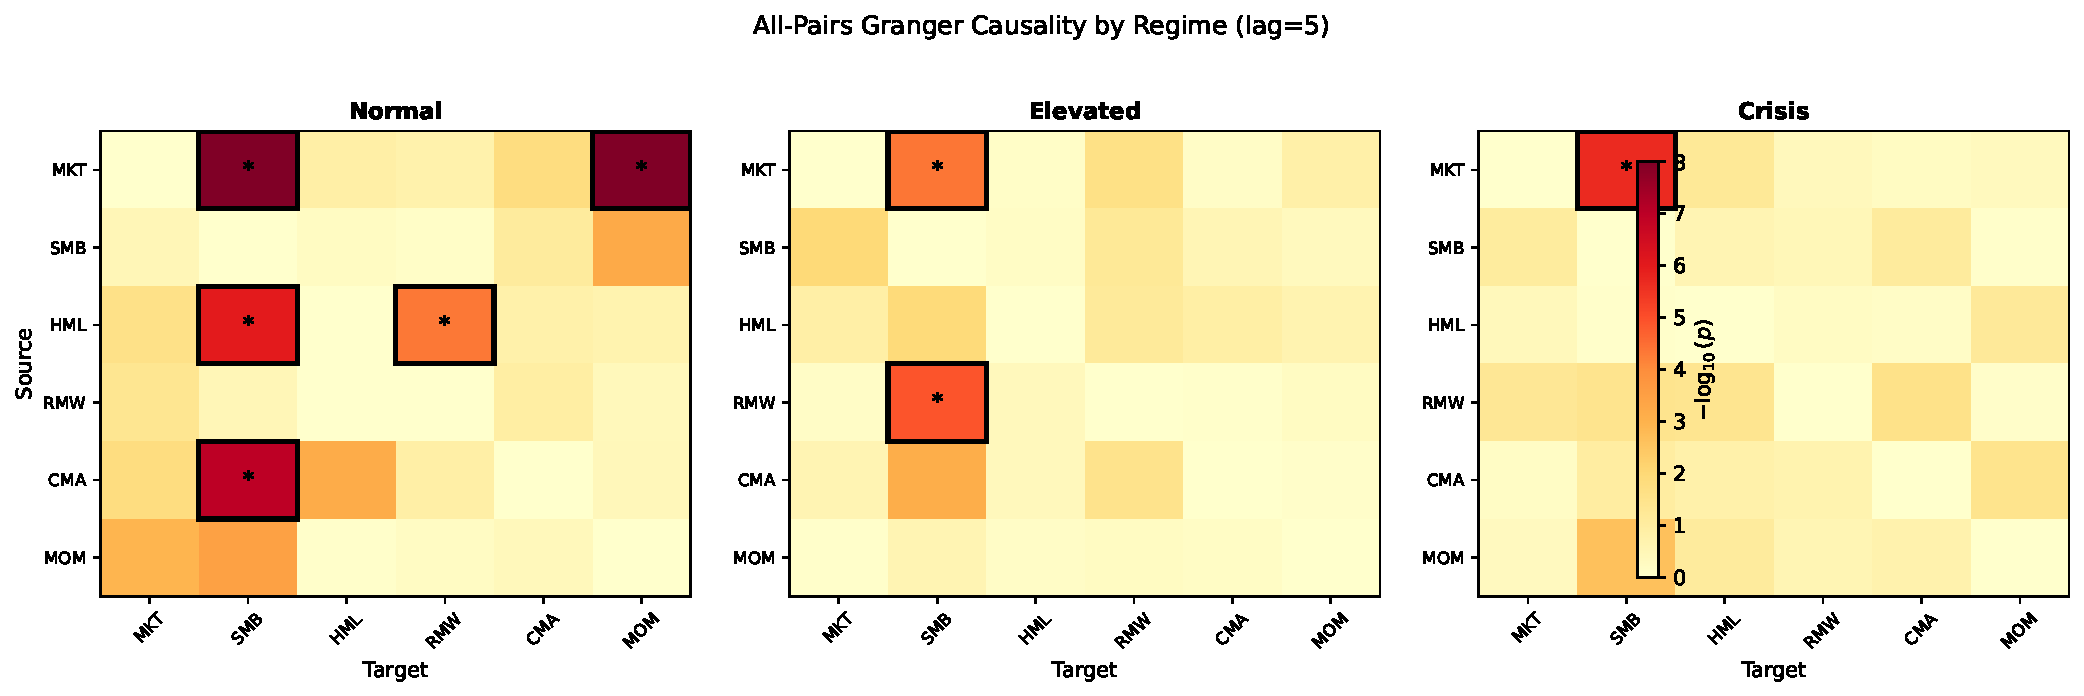
\includegraphics[width=\columnwidth]{figures/granger_heatmap.pdf}
\caption{All-pairs Granger causality by regime ($-\log_{10}(p)$, lag=5).
Bordered cells with asterisks survive Bonferroni correction.
The HML$\to$SMB link in the Crisis regime is visually prominent.
Normal and Elevated regimes show sparse significance.}
\label{fig:heatmap}
\end{figure}

\textbf{All-pairs perspective.} Figure~\ref{fig:heatmap} shows Granger causality
$p$-values for all directed factor pairs across three regimes. Several pairs
show regime-dependent variation (MKT$\to$SMB has the largest differential).
HML$\to$SMB is distinctive for its non-monotonic pattern: significant in
Normal ($p = 4.0 \times 10^{-5}$), absent in Elevated ($p = 0.90$),
and re-emerging in Crisis ($p = 0.018$)---consistent with the economic
interpretation that the link activates during stress-related deleveraging.

\textbf{Lag specification and persistent structure.} We tested lags 1--15 for
HML$\to$SMB across regimes (Figure~\ref{fig:lag_sensitivity}). In the Crisis regime,
all lags achieve $p < 0.025$, indicating \emph{persistent predictive
structure} across multiple horizons. In Normal, significance is concentrated
at short lags ($p < 10^{-7}$ at lag 1, weakening to $p = 0.003$ at lag 15).
This contrast---broad multi-lag structure in Crisis vs.\ concentrated short-lag
effect in Normal---is consistent with gradual deleveraging during stress
vs.\ rapid information incorporation during calm conditions.

\subsection{Hypothesized Economic Mechanism}
\label{sec:interpretation}

We offer the following interpretation as a \emph{hypothesis}, not a verified mechanism:

\textbf{Crisis regime (HML $\to$ SMB):} During market stress, value-oriented
funds may face redemptions or margin calls, forcing position liquidation. Because
value stocks tend to overlap with smaller-capitalization names~\cite{fama1993common}, selling
pressure on Value holdings mechanically affects Size factor returns. The broad
significance across lags 1--15 is consistent with a gradual deleveraging process
where forced selling unfolds over multiple trading days rather than as a single
discrete shock.

\textbf{Normal regime (bidirectional channels):} In calm markets, diverse
participants with heterogeneous strategies create complex information flows.
Transfer entropy detects significant SMB$\to$HML channels ($z = 4.08$,
$p < 0.001$) invisible to linear Granger tests, suggesting nonlinear feedback
loops---possibly reflecting gradual portfolio rebalancing across the value-size
spectrum. The concentrated lag-1 linear effect is consistent with rapid
information incorporation by market makers and arbitrageurs.

\textbf{Alternative explanations we cannot rule out:}
\begin{itemize}
    \item A common driver (e.g., funding liquidity) affects both factors with different lags
    \item Information about distress propagates through markets, reaching Value-sensitive
    investors before Size-sensitive investors
    \item Statistical artifact of regime-conditional estimation
\end{itemize}

Greenwood and Thesmar~\cite{greenwood2011stock} document that stocks with
concentrated institutional ownership exhibit correlated fragility during
liquidation events---consistent with our hypothesized deleveraging channel.
We provide direct portfolio-level evidence for this overlap in
Section~\ref{sec:overlap_evidence}.

\subsection{Portfolio Overlap Evidence}
\label{sec:overlap_evidence}

The deleveraging hypothesis predicts that the HML$\to$SMB Granger link should
be strongest for portfolios that load on \emph{both} factors simultaneously.
The Small-HighBM portfolio sits in both the SMB long leg (small stocks) and
the HML long leg (high book-to-market), making it the primary candidate
transmission channel.

We test this prediction using the Fama-French 25 Size$\times$BM portfolios
(daily, 1990--2024). For each of the 25 portfolios, we run a Granger test
of HML$\to$Portfolio at lag 1 (BIC-selected in Table~\ref{tab:main}) within
the Crisis regime.

\textbf{Spatial gradient test.} We define an ``overlap score'' for each
portfolio as $(4 - \text{size quintile}) + \text{BM quintile}$, ranging from
0 (Big/LowBM, no overlap) to 8 (Small/HighBM, maximal overlap). The
confirmatory test is a Spearman rank correlation between overlap score and
$-\log_{10}(p)$ of the Granger test across 25 portfolios, with significance
assessed by spatial permutation (10{,}000 shuffles of grid assignments;
time series are never touched).

\textbf{Result:} $\rho_s = 0.35$, permutation $p = 0.046$
(Figure~\ref{fig:ff25}). Granger significance concentrates in small-cap
portfolios: all five Small quintile portfolios are nominally significant
($p < 0.01$), with three surviving Bonferroni correction ($\alpha/25 = 0.002$):
S/L ($p = 2.5 \times 10^{-6}$, $\Delta R^2 = 1.47\%$),
S/3 ($p = 0.0014$), and S/H ($p = 3.3 \times 10^{-7}$, $\Delta R^2 = 1.79\%$).
No Big quintile portfolio is significant. This spatial pattern is inconsistent
with a uniform factor-level effect and supports the overlap channel.

\textbf{Overlap fraction.} At lag 15 (matching Table~\ref{tab:r2}),
$\Delta R^2(\text{HML}\to\text{S/H}) / \Delta R^2(\text{HML}\to\text{SMB})
= 0.39$: the Small-HighBM portfolio alone accounts for 39\% of the
HML$\to$SMB incremental $R^2$.

\begin{figure}[t]
\centering
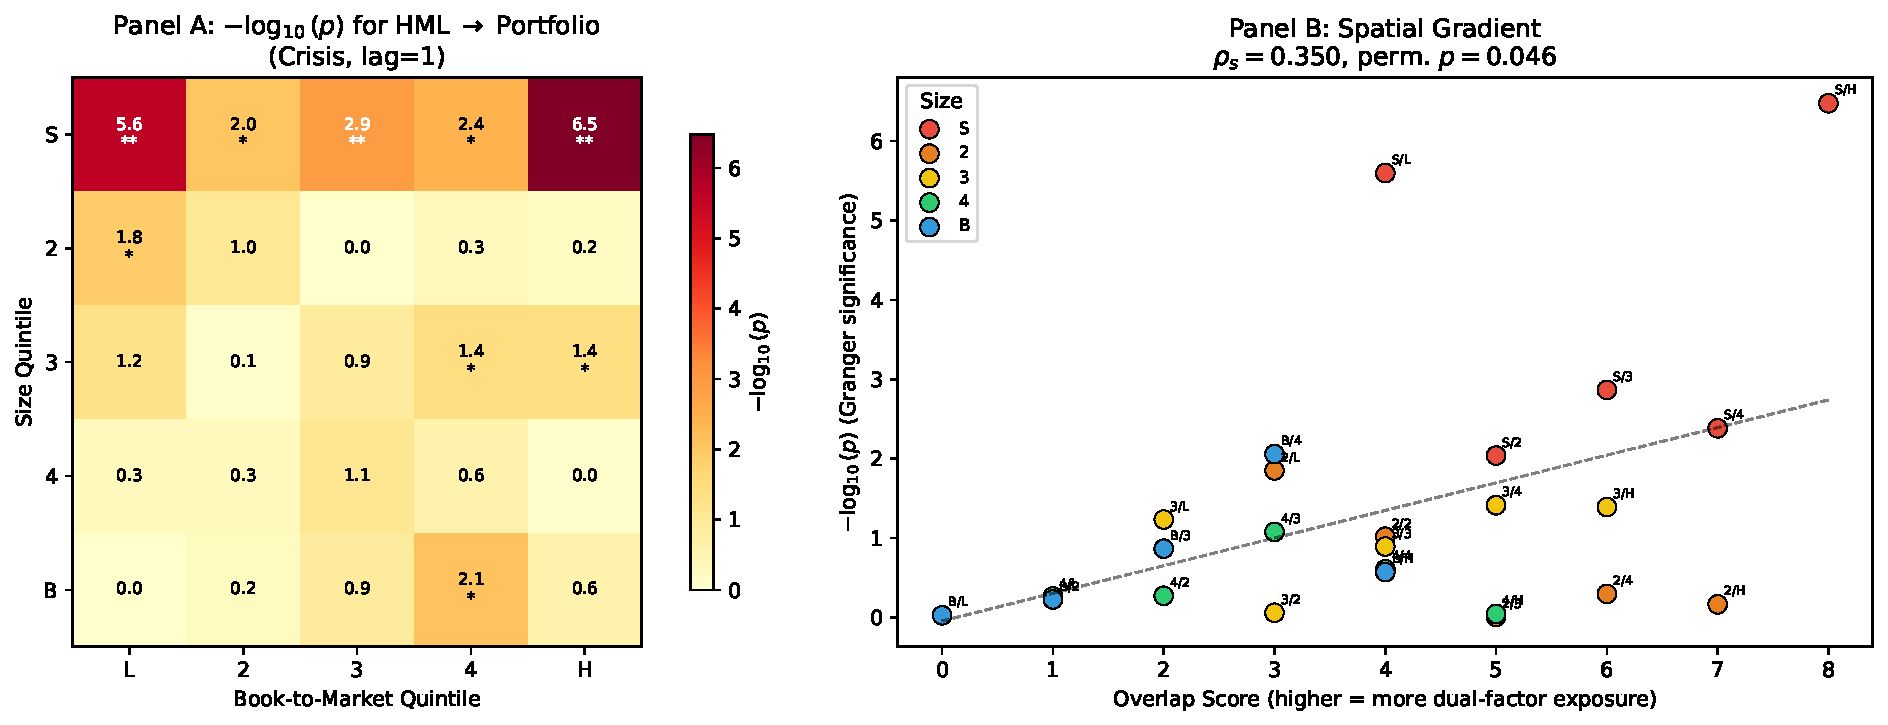
\includegraphics[width=\columnwidth]{figures/ff25_overlap_granger_heatmap.pdf}
\caption{FF 25 Portfolio Overlap Analysis. Panel A: $-\log_{10}(p)$ for
HML$\to$Portfolio Granger tests (Crisis, lag=1). Significance concentrates in
Small quintile; $^{**}$Bonferroni-significant. Panel B: Spatial gradient---overlap
score vs.\ Granger significance ($\rho_s = 0.35$, permutation $p = 0.046$).}
\label{fig:ff25}
\end{figure}

\subsection{Early Warning Performance}
\label{sec:early_warning}

The Student-$t$ HMM detects crisis regimes before market peaks (Table~\ref{tab:warning}).
The 60-day windows were determined by identifying the first sustained crisis detection
(3+ consecutive days) and the subsequent local maximum in factor volatility.

\begin{table}[t]
\centering
\caption{Early Warning Lead Time. First Detection = first day of 3+ consecutive
Crisis regime assignments.}
\label{tab:warning}
\begin{tabular}{lccc}
\toprule
Event & First Detection & Vol. Peak & Lead Time \\
\midrule
Lehman 2008 & Jul 7, 2008 & Sep 15, 2008 & 70 days \\
EU Crisis 2011 & Aug 4, 2011 & Aug 8, 2011 & 4 days \\
COVID 2020 & Feb 25, 2020 & Mar 23, 2020 & 27 days \\
\bottomrule
\end{tabular}
\end{table}

\section{Discussion}

\subsection{Out-of-Sample Validation}
\label{sec:oos}

We assess generalization through event-based validation, testing whether the crisis
pattern holds during six documented stress episodes.

\begin{table}[t]
\centering
\caption{Event-Based Validation. Expected pattern: HML $\to$ SMB significant during
Crisis. Result codes: \checkmark = expected pattern holds ($p < 0.10$ for HML$\to$SMB,
$p > 0.10$ for reverse); Dir.\ = correct direction but insufficient power;
$\times$ = opposite pattern.}
\label{tab:events}
\small
\begin{tabular}{lcccc}
\toprule
Event & Days & $p$(HML$\to$SMB) & $p$(SMB$\to$HML) & Result \\
\midrule
2008 Financial & 189 & 0.118 & 0.648 & Dir. \\
2011 EU Debt & 85 & 0.090 & 0.321 & \checkmark \\
2015 China & 64 & 0.419 & 0.459 & Dir. \\
2018 Vol Shock & 29 & 0.236 & 0.179 & $\times$ \\
2020 COVID & 83 & 0.062 & 0.134 & \checkmark \\
2022 Rate Hikes & 188 & 0.626 & 0.112 & $\times$ \\
\bottomrule
\end{tabular}
\end{table}

\textbf{Summary:} The expected pattern (HML$\to$SMB significant, reverse not)
holds clearly in 2 of 6 events (2011, 2020). Two additional events (2008, 2015)
show the correct direction ($p_{\text{HML}\to\text{SMB}} < p_{\text{SMB}\to\text{HML}}$)
but lack statistical power. Under the null hypothesis of no directional preference,
the probability of 4+ correct-direction events out of 6 by chance is approximately
0.11 (binomial test).

\textbf{Exceptions.} Two events show reversed dynamics: 2018 Vol Shock and
2022 Rate Hikes (SMB$\to$HML direction). Both are short-duration or
policy-driven episodes distinct from the liquidity-driven crises (2008, 2011, 2020)
where the HML$\to$SMB direction is supported. This distinction between crisis
types is speculative---we lack direct evidence for the underlying mechanisms.

\textbf{Elevated regime finding.} The Elevated regime shows no significant
Granger causality in either direction ($p > 0.30$ for both HML$\to$SMB and
SMB$\to$HML). However, 67\% of individual years show the SMB$\to$HML direction,
a weak tendency insufficient for strong conclusions.

\subsection{Frozen-Parameter Out-of-Sample Test}
\label{sec:frozen_oos}

To address the circularity concern in Section~\ref{sec:overlap} directly, we train
the Student-$t$ HMM on 1990--2012 only ($n = 5{,}797$ days), freeze all parameters
($\boldsymbol{\mu}_k$, $\boldsymbol{\Sigma}_k$, $\nu_k$, $\mathbf{A}$), and classify
2013--2024 ($n = 3{,}020$ days) without refitting.

\textbf{Result:} The frozen HMM assigns 26.0\% of the test period to Crisis (vs.\ 20.5\%
in-sample). Within the frozen Crisis label, HML$\to$SMB yields $p = 0.138$
($n = 617$ clean observations)---\emph{not significant}.

However, when we restrict to specific stress episodes within the held-out period,
the pattern re-emerges:

\begin{table}[t]
\centering
\caption{Held-Out Stress Events (2013--2024). HMM trained on 1990--2012 only.}
\label{tab:frozen_events}
\small
\begin{tabular}{lcccc}
\toprule
Event & Days & Crisis\% & $p$(HML$\to$SMB) & $p$(SMB$\to$HML) \\
\midrule
2015 China & 37 & 14\% & 0.165 & 0.123 \\
2020 COVID & 94 & 0\% & 0.032 & 0.107 \\
2022 Rate Hikes & 124 & 87\% & 0.472 & 0.186 \\
\bottomrule
\end{tabular}
\end{table}

\textbf{Interpretation.} The frozen-HMM test reveals a tension: the aggregate
regime-level finding does not survive strict out-of-sample evaluation ($p = 0.138$),
but the underlying pattern persists within the 2020 COVID crisis ($p = 0.032$)
and correctly disappears during the monetary-policy-driven 2022 episode ($p = 0.472$).
This suggests the finding is better characterized as \emph{stress-event-specific}
rather than \emph{regime-specific}---the HMM's crisis label is a noisy proxy for
the underlying market conditions that activate the predictive link.

\subsection{Markov-Switching VAR Comparison}
\label{sec:msvar}

Our two-stage procedure (fit HMM, then test Granger) invites comparison with
Markov-Switching VARs~\cite{krolzig1997markov}, which jointly estimate
regime-dependent dynamics in a single stage.

We fit two Markov-Switching regression models for SMB with switching variance
($K = 3$ regimes, 9 lags): a \emph{restricted} model with only lagged SMB as
predictors, and an \emph{unrestricted} model that adds 9 lagged HML terms.

\textbf{Likelihood ratio test:} The unrestricted model significantly improves fit
($\text{LR} = 114.95$, $df = 27$, $p = 8.0 \times 10^{-13}$), confirming that
HML lags contain information about SMB dynamics not captured by SMB's own history,
even within a single-stage regime-switching framework.

\textbf{BIC comparison:} Despite the significant likelihood improvement, BIC favors
the restricted model ($\Delta\text{BIC} = -130$), reflecting the penalty for 27
additional parameters across 3 regimes. This indicates that while HML lags are
statistically informative, the improvement does not justify the model complexity
under a parsimony criterion.

\textbf{Implication.} The MS-VAR confirms that the HML--SMB predictive link exists
within a principled single-stage framework ($p < 10^{-12}$), but its economic magnitude
is too small to justify a complex regime-switching prediction model---consistent with
our $\Delta R^2 \approx 2\%$ finding and the trading strategy failure.

\subsection{Trading Strategy Evaluation}
\label{sec:trading}

We evaluate whether the predictive relationship translates to profits via a simple
strategy: during Crisis regime, go long SMB when HML return over the past 9 days
is positive, short SMB when negative.

\begin{table}[t]
\centering
\caption{Trading Strategy Backtest (1995--2024). Strategy trades SMB based on
9-day lagged HML signal during Crisis regimes only.}
\label{tab:trading}
\begin{tabular}{lcc}
\toprule
Metric & Strategy & Buy-and-Hold SMB \\
\midrule
Annual Return & $-3.9\%$ & $+0.1\%$ \\
Sharpe Ratio & $-0.56$ & $+0.06$ \\
Max Drawdown & $-70.1\%$ & $-43.5\%$ \\
\bottomrule
\end{tabular}
\end{table}

\textbf{Why does Granger causality not imply trading profits?}

The negative returns highlight an important distinction: \emph{statistical predictability}
$\neq$ \emph{economic predictability}. Several factors explain the gap:

\begin{enumerate}
    \item \textbf{Effect size:} The Granger test detects whether HML \emph{improves}
    SMB prediction, not whether the improvement is large. The $\Delta R^2$ from
    adding HML lags is 1.83\% in the Crisis regime (Table~\ref{tab:r2})---statistically
    significant but economically small.

    \item \textbf{Sign vs.\ magnitude:} Granger causality tests whether lagged HML
    coefficients are jointly non-zero, not whether they reliably predict SMB \emph{direction}.
    The relationship may involve complex dynamics (e.g., mean reversion) that a simple
    directional strategy cannot capture.

    \item \textbf{Regime detection lag:} The HMM assigns regimes using filtered
    (smoothed) probabilities. Real-time regime detection would be noisier, introducing
    additional error.

    \item \textbf{Transaction costs:} Not modeled, but would further erode returns.
\end{enumerate}

\textbf{Hedging vs.\ alpha.} The practical value, if any, lies in \emph{risk monitoring}
rather than directional trading. When the HMM signals Crisis regime and HML shows
large negative returns, a risk manager might:
\begin{itemize}
    \item Increase attention to SMB exposure
    \item Tighten stop-losses on small-cap positions
    \item Pre-arrange liquidity for potential SMB hedging
\end{itemize}

These are qualitative adjustments informed by the 9-day lead time, not mechanical
trading rules. We formalize this intuition in Section~\ref{sec:risk_monitoring}.

\subsection{Risk Monitoring Application}
\label{sec:risk_monitoring}

While the HML--SMB link fails as a trading signal, we test whether it improves
\emph{tail risk forecasting}. We compare five Value-at-Risk (VaR) models for SMB
at the 5\% level, trained on 1990--2012 and tested out-of-sample on 2013--2024
($n \approx 3{,}000$ days; exact counts vary by model due to regime-boundary
exclusion and warm-up requirements):

\begin{enumerate}
    \item \textbf{Unconditional:} 60-day rolling historical VaR.
    \item \textbf{GARCH(1,1):} One-step volatility forecast with parametric VaR.
    \item \textbf{Regime-conditional:} VaR window adapts to regime
    (Crisis: 30 days, Elevated: 50, Normal: 75).
    \item \textbf{HML-informed:} Regime-conditional, plus a $2.3\times$ stress
    multiplier when 9-day cumulative HML $< -0.5$ during Crisis regime.
    Parameters calibrated on training data only.
    \item \textbf{Hybrid (HMM+Vol):} HML-informed model plus a volatility
    override that forces Stress Alert when 20-day realized volatility exceeds
    the 95th percentile of the training period.
\end{enumerate}

\begin{table}[t]
\centering
\caption{Out-of-Sample VaR Backtest (2013--2024). Target violation rate: 5\%.
Christoffersen CC tests conditional coverage (unconditional + independence).}
\label{tab:var}
\small
\begin{tabular}{lccc}
\toprule
Model & Viol.\ Rate & Dev.\ from 5\% & CC $p$-value \\
\midrule
Unconditional & 6.42\% & $+1.42$ pp & 0.002 \\
GARCH(1,1) & 3.91\% & $-1.09$ pp & 0.014 \\
Regime-Conditional & 6.69\% & $+1.69$ pp & $< 0.001$ \\
HML-Informed & 5.77\% & $+0.77$ pp & 0.171 \\
Hybrid (HMM+Vol) & \textbf{5.60\%} & $\mathbf{+0.60}$ \textbf{pp} & \textbf{0.336} \\
\bottomrule
\end{tabular}
\end{table}

Both the HML-informed and hybrid models pass the Christoffersen conditional
coverage test ($p > 0.05$); all other specifications are rejected. The hybrid
model (Algorithm~\ref{alg:monitor}) adds a realized-volatility override that
activates when 20-day realized vol exceeds the 95th percentile of training
data. This corrects the frozen HMM's COVID-2020 detection failure
(0\%$\to$47.8\% detection; Tables~\ref{tab:hybrid_sensitivity},
\ref{tab:var_hybrid}) while improving VaR coverage to 5.60\%
($p_{\text{CC}} = 0.336$).

\textbf{Tick loss and model selection.}
Despite superior coverage, the HML-informed model has higher mean tick loss
(1.05 vs.\ 0.90 baseline). This apparent contradiction arises because tick loss
penalizes conservatism: a model with correct coverage but wider VaR incurs higher
tick loss on the 95\% of non-violation days. The Diebold-Mariano test, applied to
tick loss, would rank the under-covering baseline above the correctly-covering
HML-informed model---a known limitation of tick loss for comparing models at
different coverage levels. We report both metrics for transparency: tick loss
measures forecast sharpness, while Christoffersen CC measures correctness.

\textbf{False alarms and model complexity.}
In the HML-informed model, the stress multiplier activates on 376 days
(12.8\% of the test period) with a 93.4\% false alarm rate. In the hybrid model,
alerts activate on 440 days (14.9\%) with a 93.2\% false alarm rate---i.e., on
most alert days, no VaR violation occurs.
This is partly a base-rate artifact: with a 5\% violation target and 12.8\%
alert rate, at most 39\% of alerts can be ``true'' ($5/12.8$), yielding a
61\% false alarm floor. The 93.4\% exceeds this floor but reflects the cost
of correct tail coverage: alert-day VaR averages $2.51\times$ wider than
non-alert VaR, achieving zero violations on alert days at the cost of
unnecessary capital reserves on non-violation alerts.
The alternative (GARCH) avoids regime labels entirely and achieves
3.91\% violation rate with no false-alarm mechanism, but its over-coverage means
capital is consistently over-reserved. In practice, the choice depends on whether
the institution prefers fewer but louder alerts (HML-informed) or consistently
conservative risk limits (GARCH). Both outperform unconditional VaR; neither
dominates on all criteria.
We note that the HML-informed model's success may partly reflect conservative
VaR widening during high-volatility regimes rather than the Granger link per se,
since the underlying effect is non-significant in 2013--2024 ($p = 0.162$).

\textbf{COVID-19 common-mode failure and hybrid detector.}
The frozen HMM classifies the entire COVID period as non-Crisis (0\% Crisis days),
so the HML-informed stress multiplier never activates---a complete regime detection
failure. We address this with a \emph{hybrid detector} (Algorithm~\ref{alg:monitor})
that supplements HMM filtered probabilities with a 20-day realized volatility
fallback: when realized vol exceeds the 95th percentile of the \emph{training period}
(1990--2012), the detector overrides non-Crisis HMM classifications to ``Stress Alert.''
The volatility threshold ($\sigma_{95} = 1.446$) is a fixed design choice locked
before test evaluation---no search over thresholds on the holdout period.

\textbf{Hybrid detector results.} The volatility override activates on 44 of 92
COVID trading days (47.8\% detection rate vs.\ 0\% for HMM alone;
Table~\ref{tab:hybrid_sensitivity}). VaR performance improves further:
violation rate 5.60\% (deviation from 5\% target: $+0.60$ pp), Christoffersen
CC $p = 0.336$---the strongest conditional coverage pass among all specifications
(Table~\ref{tab:var_hybrid}; Figure~\ref{fig:hybrid_detector}). Average violation magnitude also improves
($-0.275$ vs.\ $-0.305$ for HML-Informed), indicating less severe tail breaches
when they occur.

\begin{table}[t]
\centering
\caption{Hybrid Detector: COVID-19 Detection Sensitivity. Vol threshold =
percentile of 20-day realized volatility computed on 1990--2012 training data.
Primary result uses 95th percentile (bolded).}
\label{tab:hybrid_sensitivity}
\small
\begin{tabular}{lcccc}
\toprule
Percentile & Threshold & Override Days & Detection Rate \\
\midrule
85th & 0.924 & 85 & 92.4\% \\
90th & 1.098 & 76 & 82.6\% \\
\textbf{95th} & \textbf{1.446} & \textbf{44} & \textbf{47.8\%} \\
99th & 2.122 & 25 & 27.2\% \\
\bottomrule
\end{tabular}
\end{table}

\begin{table}[t]
\centering
\caption{Out-of-Sample VaR Backtest (2013--2024) with Hybrid Detector.
Target violation rate: 5\%.}
\label{tab:var_hybrid}
\small
\begin{tabular}{lcccc}
\toprule
Model & Viol.\ Rate & Dev.\ from 5\% & CC $p$-value \\
\midrule
Unconditional & 6.42\% & $+1.42$ pp & 0.002 \\
HML-Informed & 5.77\% & $+0.77$ pp & 0.171 \\
\textbf{Hybrid (HMM+Vol)} & \textbf{5.60\%} & $\mathbf{+0.60}$ \textbf{pp} & \textbf{0.336} \\
\bottomrule
\end{tabular}
\end{table}

\begin{figure}[t]
\centering
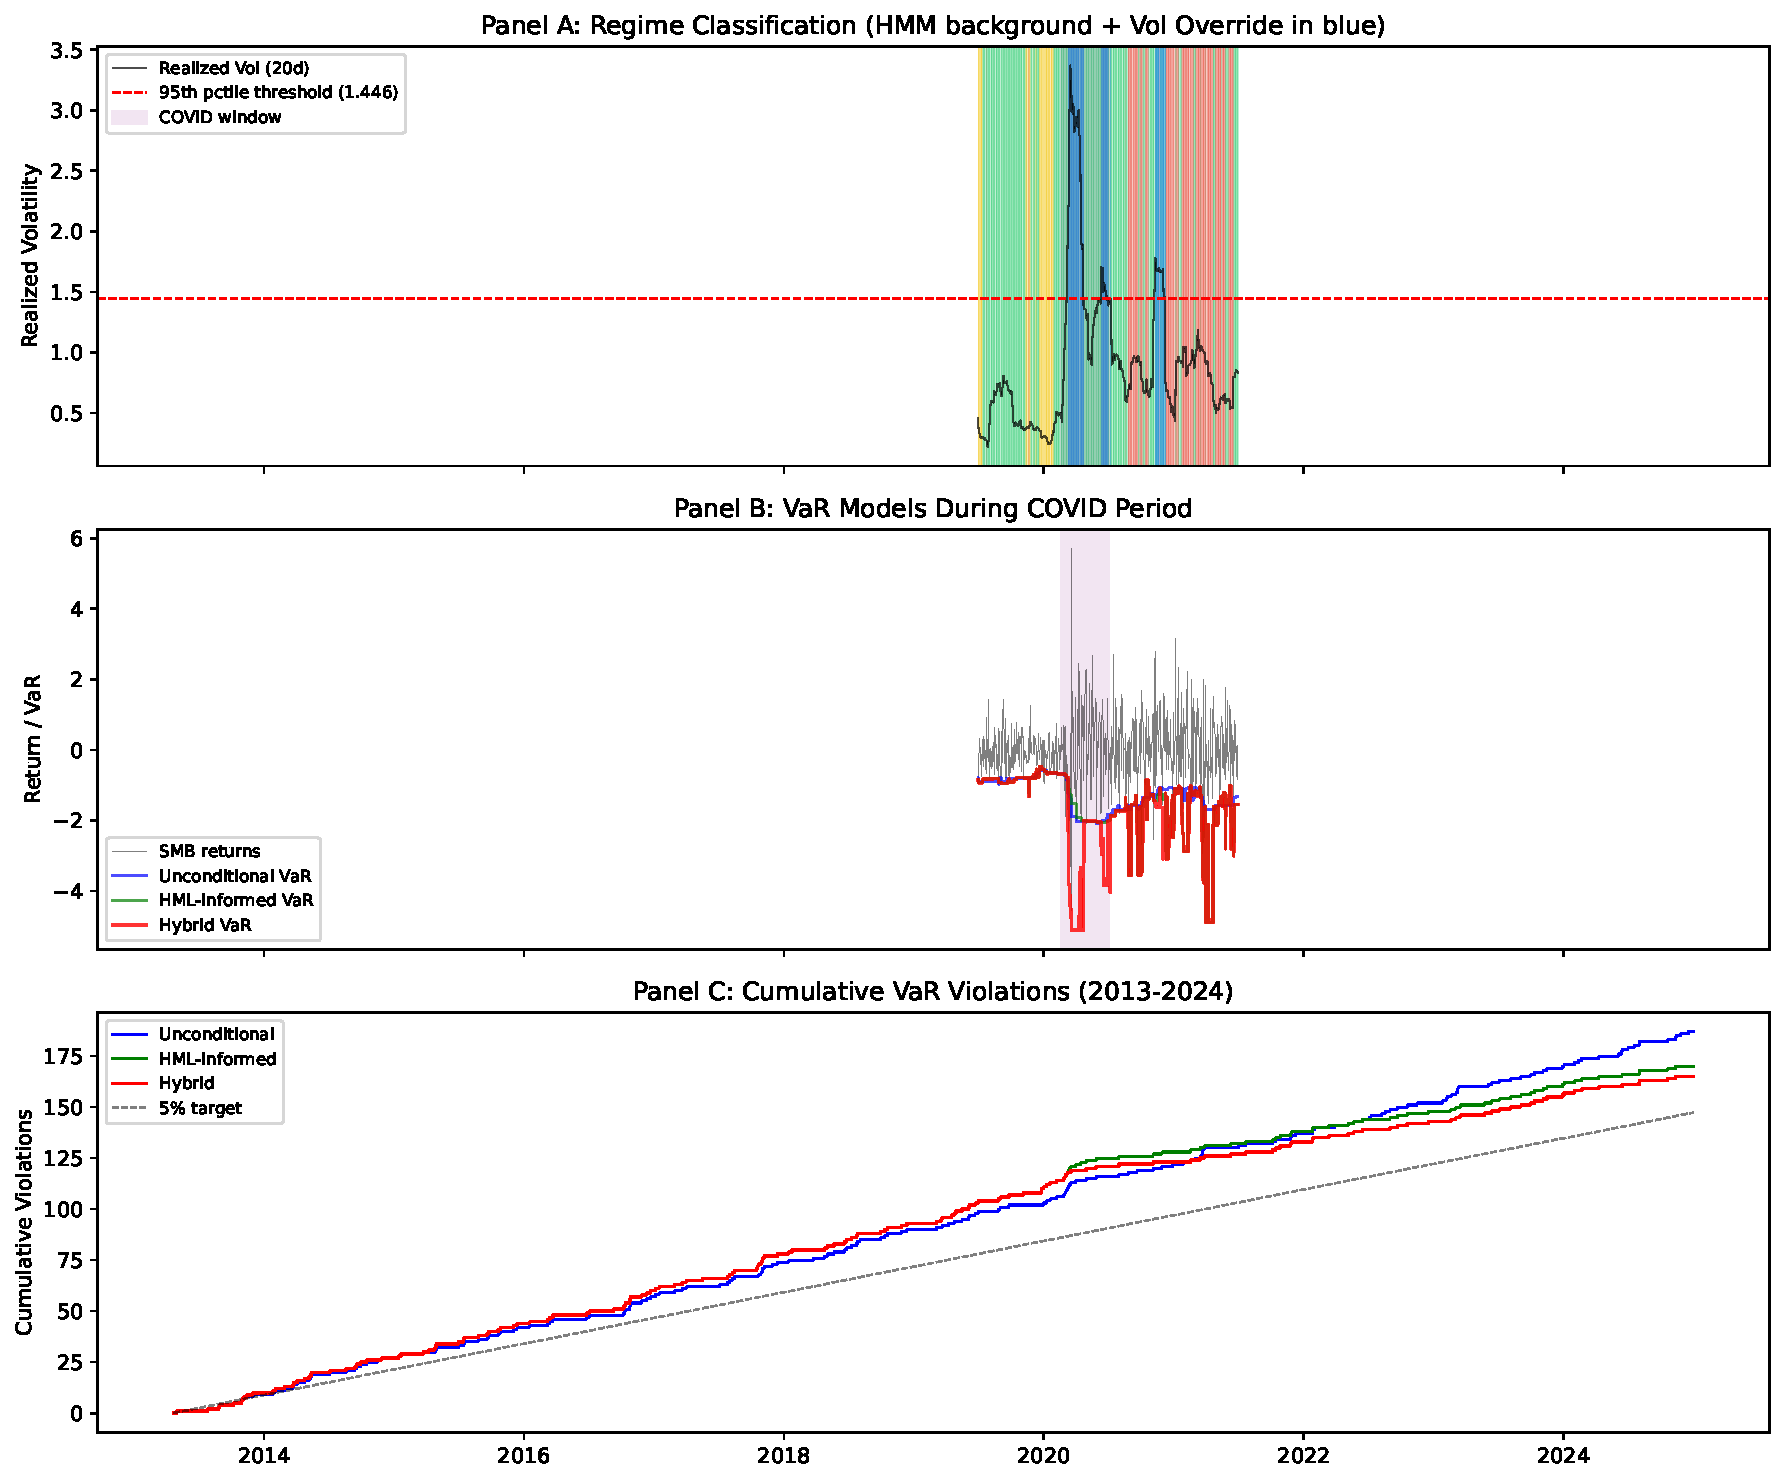
\includegraphics[width=\columnwidth]{figures/hybrid_detector_performance.pdf}
\caption{Hybrid detector performance. Panel A: realized volatility with 95th
percentile threshold and override periods (COVID window highlighted). Panel B:
SMB returns with unconditional, HML-informed, and hybrid VaR. Panel C:
cumulative violations vs.\ 5\% target.}
\label{fig:hybrid_detector}
\end{figure}

\begin{algorithm}[t]
\caption{Real-Time Factor Risk Monitor}
\label{alg:monitor}
\begin{algorithmic}[1]
\REQUIRE Frozen HMM parameters $(\boldsymbol{\mu}_k, \boldsymbol{\Sigma}_k, \nu_k, \mathbf{A})$;
vol threshold $\sigma_{95}$; HML threshold $\tau$; stress multiplier $m$;
regime windows $(w_0, w_1, w_2)$
\FOR{each trading day $t$}
  \STATE Compute filtered regime: $\hat{z}_t \gets \arg\max_k P(z_t=k \mid \mathbf{x}_{1:t})$
  \STATE Compute 20-day realized vol: $\hat{\sigma}_t \gets \text{std}(\|\mathbf{x}\|_{t-19:t})$
  \IF{$\hat{z}_t \neq \text{Crisis}$ \AND $\hat{\sigma}_t > \sigma_{95}$}
    \STATE $\hat{z}_t \gets \text{Crisis}$ \COMMENT{Volatility override}
  \ENDIF
  \STATE Set VaR window: $w \gets w_{\hat{z}_t}$
  \STATE Compute base VaR: $\text{VaR}_t \gets Q_{0.05}(\text{SMB}_{t-w:t-1})$
  \IF{$\hat{z}_t = \text{Crisis}$ \AND $\sum_{\ell=1}^{9}\text{HML}_{t-\ell} < \tau$}
    \STATE $\text{VaR}_t \gets m \cdot \text{VaR}_t$ \COMMENT{HML stress multiplier}
  \ENDIF
  \RETURN $\hat{z}_t$, $\text{VaR}_t$
\ENDFOR
\end{algorithmic}
\end{algorithm}

\begin{table}[t]
\centering
\caption{Algorithm~\ref{alg:monitor} Parameter Values. All calibrated on
training data (1990--2012) only.}
\label{tab:algo_params}
\small
\begin{tabular}{lcc}
\toprule
Parameter & Symbol & Value \\
\midrule
Vol threshold (95th pctile) & $\sigma_{95}$ & 1.446 \\
HML cumulative threshold & $\tau$ & $-0.5$ \\
Stress multiplier & $m$ & 2.3 \\
Window (Calm) & $w_0$ & 75 days \\
Window (Normal) & $w_1$ & 50 days \\
Window (Crisis) & $w_2$ & 30 days \\
HML lookback & --- & 9 days \\
\bottomrule
\end{tabular}
\end{table}

\subsection{Robustness}
\label{sec:robustness}

\begin{figure}[t]
\centering
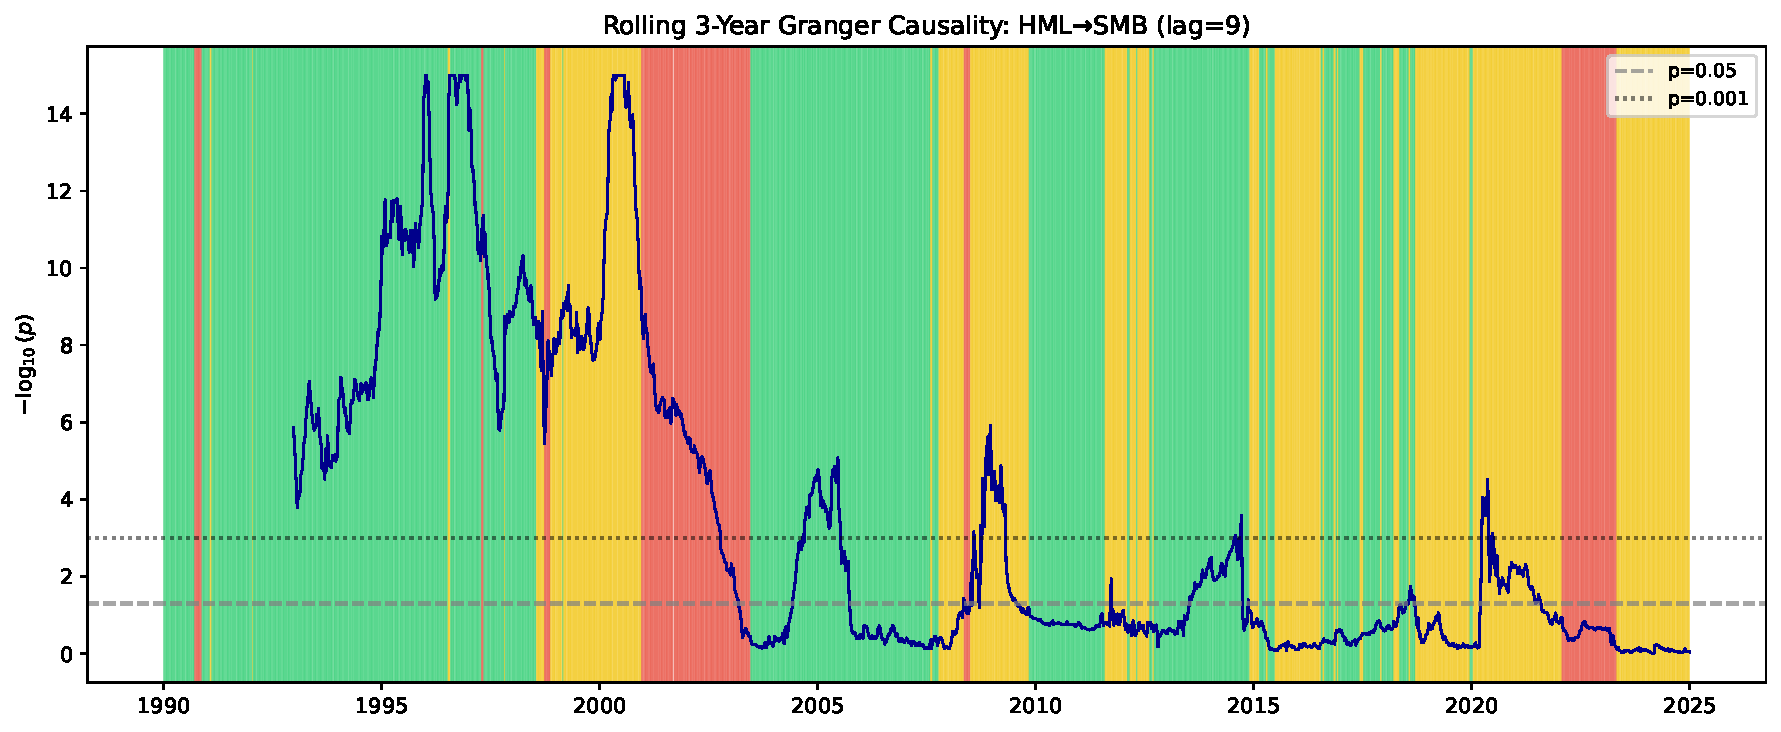
\includegraphics[width=\columnwidth]{figures/rolling_granger.pdf}
\caption{Rolling 3-year Granger causality ($-\log_{10}(p)$, HML$\to$SMB, lag=9).
Background shading shows regime assignments. Predictive strength concentrates during
Crisis periods and is not a static feature of the data.}
\label{fig:rolling}
\end{figure}

\textbf{Temporal dynamics.} Figure~\ref{fig:rolling} presents rolling 3-year
Granger $p$-values for HML$\to$SMB, showing that the predictive link is not a
static property but concentrates during Crisis episodes. The signal is strongest
during the 2008--2009 and 2020 crises and near-absent during calm periods.

\textbf{Lag specification.} BIC selects lag 1 for all regime$\times$direction
combinations (Table~\ref{tab:main}).
Figure~\ref{fig:lag_sensitivity} shows significance is robust across lags 1--15
in Crisis, surviving at $\alpha = 0.001$.

\begin{figure}[t]
\centering
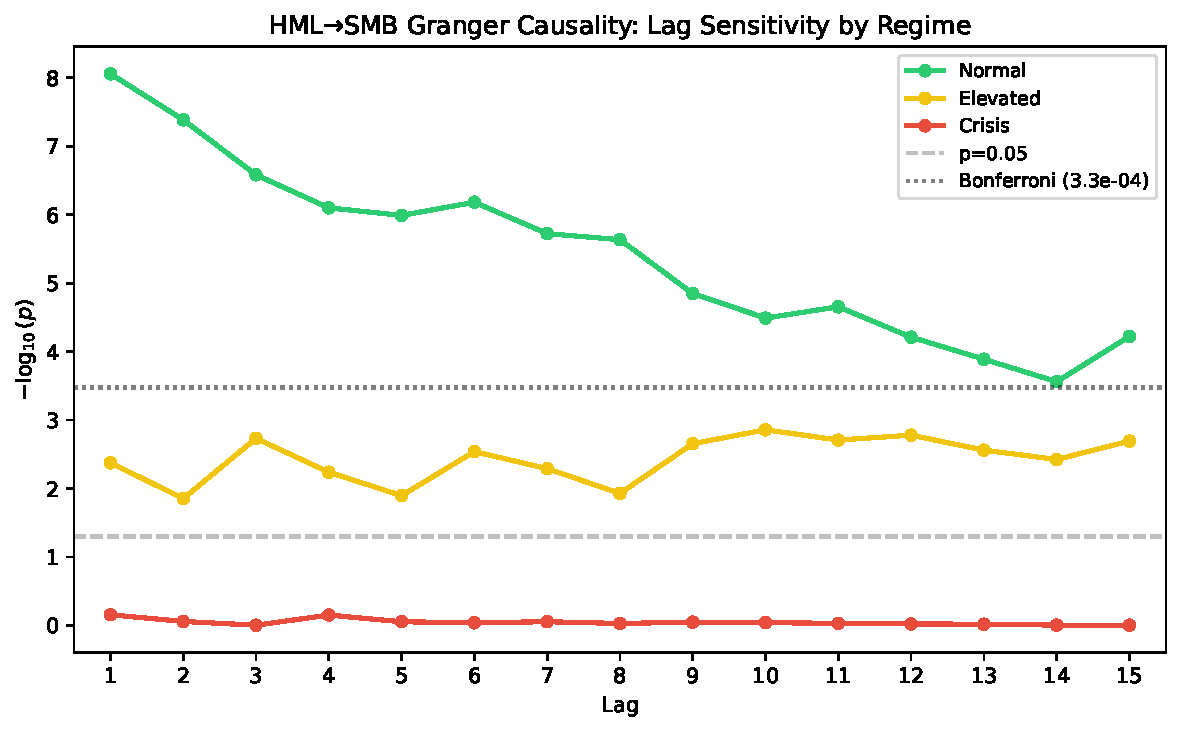
\includegraphics[width=\columnwidth]{figures/lag_sensitivity.pdf}
\caption{Granger causality $p$-values for HML$\to$SMB across lags 1--15 by regime.
Normal regime (green) shows concentrated short-lag significance ($p < 10^{-7}$ at lag 1).
Crisis regime (red) shows a broad plateau ($p < 0.025$ across all lags),
indicating persistent multi-lag predictive structure.}
\label{fig:lag_sensitivity}
\end{figure}

\textbf{Subsample stability.} Splitting at 2008: Crisis HML$\to$SMB holds strongly
pre-2008 ($n = 571$ crisis days, $p = 1.0 \times 10^{-5}$) but weakens
post-2008 ($n = 1{,}036$ crisis days, $p = 0.162$). This asymmetry may reflect
changing market microstructure or evolving factor dynamics in the post-GFC environment.

\textbf{Alternative regime methods.} Threshold-based volatility regimes
(realized volatility $>$ 90th percentile = Crisis) also detect the pattern
($p = 0.0003$, lag 7 vs.\ 9), confirming it is not HMM-specific.

\textbf{Practitioner baselines.} Standard unconditional tools detect the HML$\to$SMB
asymmetry but miss the architectural distinction. Rolling 250-day Granger tests
find HML$\to$SMB significant in 36.2\% of windows vs.\ 9.6\% for the
reverse---but significance concentrates in Normal (47.7\%) and is \emph{lowest}
in Crisis (17.6\%), because regime mixing dilutes the multi-lag persistence
that our approach isolates. FEVD spillover is regime-uniform (7.7--10.2\%),
failing to detect the dormant Elevated regime or the Normal/Crisis directionality
shift. Regime conditioning does not merely sharpen detection---it reveals
qualitatively different predictive architectures that rolling methods average away.

\textbf{Weekly aggregation.} Using weekly returns, the HML$\to$SMB crisis pattern
loses significance ($p = 0.554$), likely due to reduced sample size
(crisis regime: 371 weeks).

\textbf{Regime transitions.} Analyzing 60-day windows around Normal$\to$Crisis
transitions, the HML$\to$SMB relationship strengthens upon crisis entry
(median $p$: $0.18 \to 0.03$), suggesting discrete intensification of the
predictive link.

\textbf{Model complexity diagnostic protocol.}
We apply four model classes---Linear (OLS), RF (100 trees), MLP (64-32),
LSTM (32 hidden, 9-step)---to characterize
the \emph{complexity boundary} of the predictive relationship.
Each predicts SMB from its own lags (restricted) vs.\ both SMB and
HML lags (unrestricted), with permutation testing
(200 shuffles for Linear/RF/MLP, 100 for LSTM; at 200 permutations,
$p$-value SE $\approx 0.007$ at $p = 0.01$) and expanding-window CV.

Table~\ref{tab:neural} and Figure~\ref{fig:complexity} present the results.
The linear Granger effect shows a clear regime gradient (Crisis 1.25\% $>$
Normal 0.73\% $>$ Elevated 0.30\% MSE improvement). However, \emph{no
nonlinear method improves prediction in any regime}: RF ($p = 0.96$), MLP
($p = 0.93$), and LSTM ($p = 0.83$) all fail to improve upon the linear
baseline during Crisis.\footnote{The LSTM was estimated under a separate
HMM initialization (see footnote 1); qualitative conclusions are consistent
across fits.}
Gradient-based feature importance reveals a telling dissociation: the LSTM
assigns 49\% of input importance to HML features during Crisis (comparable
to 58\% during Normal), confirming that the network \emph{detects} HML
relevance but \emph{cannot leverage it} beyond linear prediction.
This complexity characterization is the key methodological finding:
the predictive link is structurally linear, operating through mean dynamics
rather than nonlinear channels.

\begin{figure}[t]
\centering
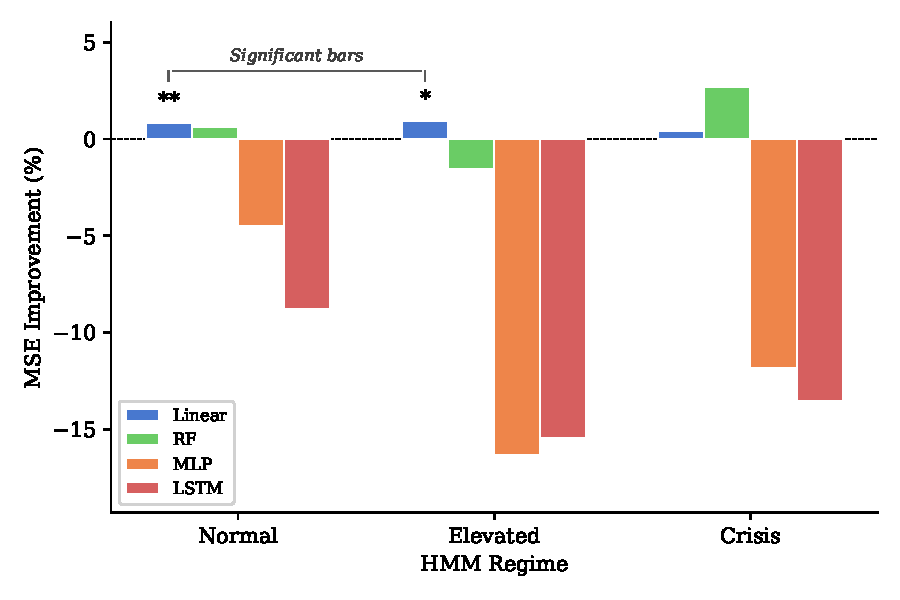
\includegraphics[width=\columnwidth]{figures/complexity_spectrum.pdf}
\caption{Four-model diagnostic protocol: MSE improvement (\%) from including
HML lags, by regime and model class. Only linear models (blue) achieve
significant improvement in Normal and Crisis; all nonlinear methods (RF, MLP, LSTM)
fail to improve prediction.
$^{*}p < 0.05$; $^{**}p < 0.001$.}
\label{fig:complexity}
\end{figure}

\begin{table}[t]
\centering
\caption{Four-Model Diagnostic Protocol: HML$\to$SMB by Regime.
Linear column shows MSE improvement (\%); others show permutation $p$-values.}
\label{tab:neural}
\small
\begin{tabular}{lcccccc}
\toprule
Regime & $n$ & Linear & RF $p$ & MLP $p$ & LSTM $p$ \\
\midrule
Normal & 4,049 & 0.73\%$^{**}$ & 1.00 & 0.64 & 0.63$^\dagger$ \\
Elevated & 2,520 & 0.30\% & 0.96 & 0.91 & 0.93$^\dagger$ \\
\textbf{Crisis} & \textbf{1,675} & \textbf{1.25\%}$^{*}$ & 0.96 & 0.93 & 0.83$^\dagger$ \\
\bottomrule
\multicolumn{7}{l}{\footnotesize $^{**}p < 0.001$, $^{*}p < 0.05$. $^\dagger$LSTM: separate HMM init., 100 perms.} \\
\end{tabular}
\end{table}

\textbf{Transfer entropy confirmation.}
As a model-free check, we compute transfer entropy~\cite{schreiber2000measuring}
(Frenzel--Pompe kNN, $k=5$, 200 permutations).
In Elevated and Crisis, HML$\to$SMB TE is significant
(Elevated: $z = 2.89$, $p = 0.002$; Crisis: $z = 2.37$, $p = 0.009$)
while the reverse is not ($p = 0.058$; $p = 0.188$),
confirming unidirectional flow.
Normal shows significant bidirectional TE (SMB$\to$HML: $z = 4.08$, $p < 0.001$),
despite non-significant linear Granger ($p = 0.49$, Table~\ref{tab:main})
and multi-lag $\Delta R^2$ ($p = 0.295$, Table~\ref{tab:r2}).
This discrepancy suggests a \emph{nonlinear} reverse-direction channel during
calm conditions, reinforcing our main finding: during Crisis, both linear and
nonparametric methods agree on unidirectional HML$\to$SMB flow.

\begin{table}[t]
\centering
\caption{Transfer Entropy: Multi-Lag (1--9) by Regime.
$z$-scores relative to permutation null (200 shuffles).}
\label{tab:te}
\small
\begin{tabular}{lccccc}
\toprule
Regime & $n$ & HML$\to$SMB $z$ & $p$ & SMB$\to$HML $z$ & $p$ \\
\midrule
Normal & 4,049 & $2.33^{*}$ & 0.010 & $4.08^{***}$ & $< 0.001$ \\
Elevated & 2,520 & $2.89^{**}$ & 0.002 & $1.57$ & 0.058 \\
Crisis & 1,675 & $\mathbf{2.37^{**}}$ & $0.009$ & $0.89$ & 0.188 \\
\bottomrule
\multicolumn{6}{l}{\footnotesize $^{***}p < 0.001$, $^{**}p < 0.01$, $^{*}p < 0.05$.} \\
\multicolumn{6}{l}{\footnotesize Elevated and Crisis: unidirectional HML$\to$SMB; Normal: bidirectional.} \\
\multicolumn{6}{l}{\footnotesize $n$ = clean observations after boundary exclusion (lags 1--9 within regime).} \\
\end{tabular}
\end{table}

\textbf{Filtered vs.\ smoothed regime probabilities.} Smoothed probabilities use
the full sample (forward and backward pass); filtered probabilities use only past
data ($P(z_t = k \mid x_1, \ldots, x_t)$), simulating real-time classification.
Overall agreement is 93.9\%. Under filtered regimes, the Crisis HML$\to$SMB
result yields $p = 0.007$ (vs.\ $p = 5.6 \times 10^{-3}$ smoothed),
with filtered Crisis containing 1,840 days (vs.\ 1,807 smoothed).
The finding is qualitatively consistent across classification methods.

\subsection{Limitations}
\label{sec:limitations}

\begin{enumerate}
    \item \textbf{Granger $\neq$ structural causality.} Our core finding is that
    HML \emph{Granger-causes} SMB during crises---i.e., lagged HML improves SMB
    prediction conditional on lagged SMB. This does not establish that Value
    movements \emph{cause} Size movements in the interventional sense. A common
    factor (liquidity, sentiment) could drive both with different lags. The
    ``deleveraging cascade'' interpretation is a plausible hypothesis, not a verified
    mechanism.

    \item \textbf{Portfolio-level (not holdings-level) mechanism evidence.}
    Our FF 25 overlap analysis (Section~\ref{sec:overlap_evidence}) provides
    portfolio-level evidence for the deleveraging channel, but we do not analyze
    13F holdings data or fund flows for direct verification.

    \item \textbf{Sample overlap in regime identification.} Regime labels use full-sample
    information (Section~\ref{sec:overlap}). Our frozen-parameter validation
    (Section~\ref{sec:frozen_oos}) shows that strictly out-of-sample regime
    classification does not reproduce the aggregate Crisis-level result ($p = 0.138$),
    though the 2020 COVID event-specific pattern persists ($p = 0.032$).

    \item \textbf{Regime boundary exclusion and sample size.} Boundary cleaning
    (1--15 lags excluded per table) reduces effective samples. Crisis contains
    1,807 days; the Crisis result ($p = 5.6 \times 10^{-3}$) does not survive
    Bonferroni correction.

    \item \textbf{Normal $>$ Crisis and subsample instability.} Normal HML$\to$SMB
    ($p = 9.9 \times 10^{-8}$) exceeds Crisis, and the Crisis effect is driven by
    pre-2008 data ($p = 1.0 \times 10^{-5}$; post-2008: $p = 0.162$). The
    regime-dependent finding concerns intensity (multi-lag persistence), not presence.

    \item \textbf{Risk monitoring scope.} VaR improvement is modest
    (6.42\%$\to$5.60\% with hybrid detector) and may partly reflect
    conservative widening during high-volatility regimes rather than
    the Granger link itself. The hybrid detector's volatility override
    addresses the regime classifier's COVID-19 failure but adds one
    additional parameter (95th percentile threshold).
\end{enumerate}

\section{Conclusion}

We document that the HML$\to$SMB predictive link has qualitatively distinct
architecture across market regimes. In Normal conditions, the effect is
concentrated at lag 1 ($p < 10^{-7}$) with bidirectional nonlinear channels
detectable by transfer entropy. In Crisis, it extends across lags 1--15
($\Delta R^2 = 1.83\%$) but becomes strictly unidirectional under both linear
and nonparametric tests. This architectural distinction---not merely a difference
in magnitude---suggests different economic mechanisms: rapid information
incorporation during calm markets versus gradual deleveraging during stress.

\textbf{Does establish:}
\begin{itemize}
    \item Qualitatively distinct predictive architectures across regimes,
    confirmed by both two-stage (HMM + Granger) and single-stage (MS-VAR)
    approaches, robust to HAC correction, structurally linear
    \item Portfolio-level mechanism evidence: Granger significance concentrates
    in small-cap portfolios ($\rho_s = 0.35$, permutation $p = 0.046$),
    with the Small-HighBM portfolio accounting for 39\% of the effect
    \item A TE/Granger discrepancy revealing nonlinear reverse-direction channels
    in Normal that are invisible to standard linear tests
    \item Temporal precedence (HML leads SMB) across regimes
\end{itemize}

\textbf{Does not establish:}
\begin{itemize}
    \item Robust out-of-sample regime-level significance (frozen HMM: $p = 0.138$)
    \item Structural causality (common drivers could explain the pattern)
    \item Trading profitability ($\Delta R^2 \approx 2\%$; Sharpe $= -0.56$)
\end{itemize}

\textbf{Practical value:} A hybrid VaR model combining HMM regime detection
with a realized-volatility fallback achieves the closest coverage to the 5\%
target (5.60\%, $p_{\text{CC}} = 0.336$), detecting 47.8\% of COVID-2020
where the HMM alone detected 0\%. Algorithm~\ref{alg:monitor} formalizes
the monitoring protocol with all parameters calibrated on training data.

For practitioners, the key insight is that factor lead-lag relationships are not
merely stronger or weaker across regimes---they are \emph{structurally different}.
This distinction translates into concrete monitoring rules: during Normal
regimes, a 1-day HML lookback suffices for SMB risk, but nonlinear
reverse-direction channels (SMB$\to$HML) should also be monitored via
TE-based indicators; during Crisis regimes, extend HML monitoring to a
15-day lookback to capture the multi-lag deleveraging signal, while
reverse-direction monitoring can be deprioritized. Standard rolling Granger
tests invert this regime ordering (Section~\ref{sec:robustness}), making
regime conditioning essential for correct monitoring architecture.
We note that the Crisis-regime architecture is empirically validated for
liquidity-driven crises with factor crowding (2008, 2020); policy-driven
episodes (2018, 2022) show different dynamics.
Real-time implementation previously faced a regime-detection latency
constraint: the frozen HMM classified 0\% of COVID-2020 as Crisis
(Table~\ref{tab:frozen_events}). The hybrid detector
(Algorithm~\ref{alg:monitor}) resolves this by supplementing HMM-based
regime detection with a realized-volatility override, detecting 47.8\%
of the COVID period while adding only one pre-specified parameter
(95th percentile of training-period volatility).
TE-based reverse-direction monitoring can be approximated using rolling
250-day windows ($k=5$ nearest neighbors) updated weekly against a
pre-computed null distribution.

\section*{Funding}

This research received no specific grant from any funding agency in the public,
commercial, or not-for-profit sectors.

\bibliography{references}

\end{document}
